\documentclass[11pt, oneside]{article} 
\usepackage{geometry}
\geometry{letterpaper} 
\usepackage{graphicx}
	
\usepackage{amssymb}
\usepackage{amsmath}
\usepackage{parskip}
\usepackage{color}
\usepackage{hyperref}

\graphicspath{{/Users/telliott/Github/number_theory/png/}}
% \begin{center} \includegraphics [scale=0.4] {gauss3.png} \end{center}

\title{Quotient remainder rule}
\date{}

\begin{document}
\maketitle
\Large

Given integer $a$ and positive integer $b$, there exist unique positive integers $q$ and $r$ such that
\[ a = b \cdot q + r \]
with $0 \le r < b$.

This works for integer $a$, but it's easier to think about if we restrict things to $a > 0$.

Then, this is a version of the Archimedean property for positive integers.  

\begin{center} 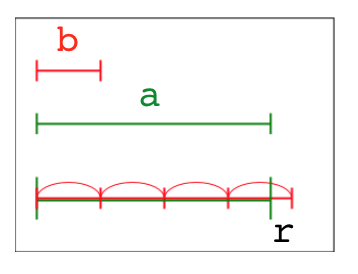
\includegraphics [scale=0.4] {Archimedean_property2.png} \end{center}
We can paraphrase by saying
\begin{quote}given a bathtub full of water and a teaspoon, it is possible to empty the bathtub.\end{quote}

First, find $q$ such that $b \cdot q \le a$ but $(b + 1) \cdot q$ produces a number larger than $a$.

Then either $b \cdot q = a$ and we are done or:

\[ b \cdot q < a < b \cdot q + b \]
So then let $r = a - bq$ and we have found
\[ 0 \le r < b \]

with $0 \le r < b$.

\subsection*{second proof}

A formal proof of this is surprisingly long-winded.  Here is one version.  

\url{https://math.stackexchange.com/questions/724032/quotient-remainder-theorem-proving}

Consider the progression:
\[ a - 3b, a - 2b, a - b, a, a + b, a + 2b, a + 3b \]

This extends in both directions.  By the well-ordering principle, there must exist a smallest non-negative element, $r$.  Thus
\[ r = a - qb \]
for some integer $q$.

$r$ must be in the interval $[0,b)$ because otherwise $r-b$ would be smaller than $r$ and a non-negative element in the progression.

\subsection*{uniqueness}
We have
\[ a = bq + r \]
with $0 \le r < b$.

Suppose we have another $q'$ and $r'$ such that
\[ a = bq' + r' \]
with $0 \le r' < b$.

Subtracting, we see that
\[ 0 = bq - bq' + r - r' \]
\[ r - r' = b(q' - q) \]

We conclude that $b | (r - r')$.

The largest value for $r - r'$ occurs when $r = b -1$ and $r' = 0$ so, at most
\[ r - r' < b \]

whereas at least (with $r = 0$)
\[ -b < r - r' \]

so then we have that $-b < r - r' < b$.  

Hence, since $b | (r - r')$, we must have that $r - r' = 0$.  

So
\[ r = r' \]
and thus
\[ r - r' = 0 = b(q' - q) \]
so 
\[ q = q' \]

The original solution is unique.

$\square$


\end{document}